\newpage

\section{Class \tkzClass{conic}}
The variable \tkzVar{conic}{CO} holds a table used to store conics. It is optional, and you are free to choose the variable name. However, using \tkzVar{conic}{CO} is a recommended convention for clarity and consistency. If you use a custom variable (e.g., \code{Conics}), you must initialize it manually. The \code{init\_elements()} function reinitializes the \tkzVar{conic}{CO} table if used.


\subsection{Preamble}
To illustrate some of the methods for working with conics, consider the construction of a parabola defined as the locus of all centers of circles tangent to a fixed circle and a line.

In the example below, the table \code{points} contains the coordinates of these centers. Since \TIKZ{} only requires a list of coordinate pairs enclosed in parentheses, the table is converted accordingly.

The table that defines the circles is slightly more elaborate. It stores, for each circle, both its center and its point of tangency with the given curve or line. Each entry is a sequence of four coordinates. These sequences are then concatenated into a string using a comma (",") as a separator.

These coordinates are finally read by \tkzMacro{TikZ}{foreach}, using the |expand list| option.

\vspace{1em}
\directlua{
z.O = point(0, 0)
z.K = point(0, 1)
z.P = point(0, 6)
z.M = point(0, 2)
z.I = point(1, 0)
C.PM = circle (z.P,z.M)
PA.center = path()
PA.through = path()
 for t = -0.24, 0.24, 0.004 do
   if (t > - 0.002 and t < 0.002) then else
       local a = C.PM : point (t)
       L.OI = line (z.O, z.I)
       L.PA = line (z.P, a)
       local c = intersection (L.OI, L.PA)
       L.tgt = C.PM : tangent_at (a)
       local x = intersection (L.tgt, L.OI)
       local o = bisector (x, a, c).pb
       PA.center:add_point(o)
       PA.through:add_point(a)
    end
  end}
\begin{center}
  \begin{tikzpicture}[scale =.5]
  \tkzGetNodes
  \tkzDrawCircles[thick, orange](P,M K,M)
  \tkzDrawCirclesFromPaths[draw,orange,thick](PA.center,PA.through)
  \tkzDrawCoordinates[smooth,red,ultra thick](PA.center)
  \end{tikzpicture}
\end{center}


Here's the code. Two paths(tables) are created, one containing the points of the parabola, the other the points that define the tangent circles.
The parabola is obtained using \TIKZ{}'s ability to draw a curve from a list of coordinates.

\begin{verbatim}
\directlua{
z.O = point(0, 0)
z.K = point(0, 1)
z.P = point(0, 6)
z.M = point(0, 2)
z.I = point(1, 0)
C.PM = circle (z.P,z.M)
PA.center = path()
PA.through = path()
 for t = -0.24, 0.24, 0.004 do
   if (t > - 0.002 and t < 0.002) then else
       local a = C.PM : point (t)
       L.OI = line (z.O, z.I)
       L.PA = line (z.P, a)
       local c = intersection (L.OI, L.PA)
       L.tgt = C.PM : tangent_at (a)
       local x = intersection (L.tgt, L.OI)
       local o = bisector (x, a, c).pb
       PA.center:add_point(o)
       PA.through:add_point(a)
    end
  end}
\end{verbatim}

\begin{verbatim}
\begin{tikzpicture}[scale =.5]
  \tkzGetNodes
  \tkzDrawCircles[thick, orange](P,M K,M)
  \tkzDrawCirclesFromPaths[draw,orange,thick](PA.center,PA.through)
  \tkzDrawCoordinates[smooth,red,ultra thick](PA.center)
\end{tikzpicture}
\end{verbatim}
This class replaces the one dedicated to ellipses. From now on, you can work with parabolas, hyperbolas and ellipses. The circle is not part of this class.
As you'll see from the examples, ellipses used to be built by \TIKZ{}, now conics are obtained by point-by-point construction. A cloud of points is sent to \TIKZ{}, which simply connects them.

\begin{mybox}
  \begin{verbatim}
    plot[<local options>]coordinates{<coordinate 1><coordinate 2>…<coordinate n>}
  \end{verbatim}
\end{mybox}

is used by the macro \tkzMacro{tkz-elements}{tkzDrawCoordinates}. One advantage of this method is that you can easily draw only part of a conic.


\subsection{Creating a Conic}
\label{sub:creating_a_conic}

The \code{conic} class unifies the construction of all classical conic sections: ellipses, parabolas, and hyperbolas. It supersedes the previously available \code{ellipse} class, which is now deprecated.

\vspace{1em}
The most natural and flexible construction method is based on the classical definition using:
\begin{itemize}
  \item a focus point,
  \item a directrix (line),
  \item and an eccentricity value \(e > 0\).
\end{itemize}

\begin{mybox}
\begin{verbatim}
CO = conic(z.F, L.dir, e)
\end{verbatim}
\end{mybox}

Depending on the value of the eccentricity:
\begin{itemize}
  \item if \(e = 1\), the result is a parabola;
  \item if \(e < 1\), an ellipse is constructed;
  \item if \(e > 1\), the result is a hyperbola.
\end{itemize}

\vspace{1em}
\paragraph{Short form.}
The class also supports a short form:
\begin{mybox}
\begin{verbatim}
CO = conic(z.F, L.dir, e)  -- equivalent to conic:new(...)
\end{verbatim}
\end{mybox}

\paragraph{Other constructions.}
Additional creation methods are also available:
\begin{itemize}
  \item Bifocal construction using two foci and a constant sum or difference;
  \item Construction from a center, vertex, and covertex;
  \item Construction from a general quadratic equation (conic coefficients).
\end{itemize}

These alternative methods are described in the following sections.



\subsection{Attributes of a conic}

Parabolas, hyperbolas, and ellipses share many attributes, though some are specific to ellipses and hyperbolas. Originally, ellipses were defined using three points: the center, a vertex, and a co-vertex. From now on, conics are preferably defined by a focus, a directrix, and an eccentricity. The old method remains available, and some tools allow conversion between both definitions.

\vspace{1em}

The key attributes for this new definition are:
\begin{itemize}
  \item \tkzAttr{conic}{Fa} : the focus,
  \item \tkzAttr{conic}{directrix} : the directrix line,
  \item \tkzAttr{conic}{e} : the eccentricity.
\end{itemize}

\vspace{1em}

A conic is the locus of all points $P$ such that the ratio of the distance to the focus $F$ over the distance to the directrix $L$ is constant and equal to $e$:

\[
\frac{PF}{PL} = e
\]

Depending on the value of $e$:
\begin{itemize}
  \item If $0 < e < 1$, the conic is an \emph{ellipse}.
  \item If $e = 1$, it is a \emph{parabola}.
  \item If $e > 1$, it is a \emph{hyperbola}.
\end{itemize}

\bgroup
  \catcode`_=12
  \small
  \captionof{table}{Conic attributes.}
  \begin{tabular}{lll}
  \toprule
  \textbf{Attributes}   & \textbf{Definition} & \textbf{Reference} \\
  \midrule
  \tkzAttr{conic}{Fa} & main foyer of the conic &\\
  \tkzAttr{conic}{directrix} & directrix of the conic &\\
  \tkzAttr{conic}{major\_axis} & Axis through focal points &\\
  \tkzAttr{conic}{minor\_axis} & Axis through focal points &\\
  \tkzAttr{conic}{e} & eccentricity of the conic &\\
  \tkzAttr{conic}{type} & The type is 'conic' &\\
  \tkzAttr{conic}{subtype} & 'parabola', 'hyperbola' or 'ellipse' &\\
  \tkzAttr{conic}{a} & Only for hyperbola and ellipse &\\
  \tkzAttr{conic}{b} & Only for hyperbola and ellipse &\\
  \tkzAttr{conic}{c} & Only for hyperbola and ellipse &\\
  \tkzAttr{conic}{p} & semi latus rectum &\\
  \tkzAttr{conic}{slope} & Slope of the line passes through the foci &\\
  \tkzAttr{conic}{K} & Projection of the focus onto the directrix &\\
  \tkzAttr{conic}{Fb} & Second focus for hyperbola and ellipse &\\
  \tkzAttr{conic}{vertex} & main vertex &\\
  \tkzAttr{conic}{covertex} & \\
  \tkzAttr{conic}{Rx} & Radius from center to vertex &\\
  \tkzAttr{conic}{Ry} & Radius from center to covertex &\\
  \bottomrule %
  \end{tabular}
  \egroup





\subsubsection{About attributes of conic}

The figure below and the associated table show common attributes and differences according to exentricity values.


\begin{verbatim}
\directlua{
 init_elements()
 z.A = point(0, 0)
 z.B = point(4, -2)
 L.dir = line(z.A, z.B)
 z.F = point(2, 2)
 CO.EL = conic(z.F, L.dir, 0.8)
 CO.PA = conic(z.F, L.dir, 1)
 CO.HY = conic(z.F, L.dir, 1.2)
 PA.EL = CO.EL:points(0, 1, 40)
 PA.PA = CO.PA:points(-5, 5, 40)
 PA.HY = CO.HY:points(-5, 5, 40)
 z.K = CO.EL.K
 z.u, z.v = CO.EL.major_axis:get()
 z.x = L.dir:report(-4, z.K)
 z.y = L.dir:report(4, z.K)
 z.r = (z.F - z.K):orthogonal(-4):at(z.F)
 z.s = (z.F - z.K):orthogonal(4):at(z.F)
 L.rs = line(z.r, z.s)
 z.I_1 = intersection(L.rs, CO.EL)
 z.I_2 = intersection(L.rs, CO.PA)
 z.I_3, _ = intersection(L.rs, CO.HY)
 z.H_1 = CO.EL.directrix:projection(z.I_1)
 z.H_2 = CO.PA.directrix:projection(z.I_2)
 z.H_3 = CO.HY.directrix:projection(z.I_3)
 z.S_2 = CO.PA.vertex
 z.F_1 = CO.EL.Fb
 z.C_1 = CO.EL.center
 z.C_3 = CO.HY.center}

\begin{tikzpicture}[scale=.8]
\tkzGetNodes
 \tkzDrawLines(x,y u,v r,s)
 \tkzDrawPoints(F,K,I_1,I_2,I_3,S_2)
 \tkzDrawPoints(H_1,H_2,H_3,F_1,C_1,C_3)
 \tkzLabelPoints(F,K,H_1,H_2,H_3,F_1,C_1,C_3)
 \tkzDrawSegments[dashed](I_1,H_1 I_2,H_2)
 \tkzDrawSegments[dashed](I_3,H_3)
 \tkzLabelPoints[above](I_1,I_2,I_3,S_2)
 \tkzDrawCoordinates[smooth](PA.EL)
 \tkzDrawCoordinates[smooth](PA.PA)
 \tkzDrawCoordinates[smooth](PA.HY)
 \tkzLabelSegment[pos=.4](K,F){$h = KF$}
 \tkzLabelSegment[sloped,pos=-.2](x,y){%
    \texttt{directrix}}
\end{tikzpicture}
\end{verbatim}

\directlua{
 init_elements()
 z.A = point(0, 0)
 z.B = point(4, -2)
 L.dir = line(z.A, z.B)
 z.F = point(2, 2)
 CO.EL = conic(z.F, L.dir, 0.8)
 CO.PA = conic(z.F, L.dir, 1)
 CO.HY = conic(z.F, L.dir, 1.2)
 PA_EL = CO.EL:points(0, 1, 40)
 PA_PA = CO.PA:points(-5, 5, 40)
 PA_HY = CO.HY:points(-5, 5, 40)
 z.K = CO.EL.K
 z.u, z.v = CO.EL.major_axis:get()
 z.x = L.dir:report(-4, z.K)
 z.y = L.dir:report(4, z.K)
 z.r = (z.F - z.K):orthogonal(-4):at(z.F)
 z.s = (z.F - z.K):orthogonal(4):at(z.F)
 L.rs = line(z.r, z.s)
 z.I_1 = intersection(L.rs, CO.EL)
 z.I_2 = intersection(L.rs, CO.PA)
 z.I_3, _ = intersection(L.rs, CO.HY)
 z.H_1 = CO.EL.directrix:projection(z.I_1)
 z.H_2 = CO.PA.directrix:projection(z.I_2)
 z.H_3 = CO.HY.directrix:projection(z.I_3)
 z.S_2 = CO.PA.vertex
 z.F_1 = CO.EL.Fb
 z.C_1 = CO.EL.center
 z.C_3 = CO.HY.center}

\begin{center}
\begin{tikzpicture}[scale=.5]
  \tkzGetNodes
  \tkzDrawLines(x,y u,v r,s)
  \tkzDrawPoints(F,K,I_1,I_2,I_3,S_2,H_1,H_2,H_3,F_1,C_1,C_3)
  \tkzLabelPoints(F,K,H_1,H_2,H_3,F_1,C_1,C_3)
  \tkzDrawSegments[dashed](I_1,H_1 I_2,H_2 I_3,H_3)
  \tkzLabelPoints[above](I_1,I_2,I_3,S_2)
  \tkzDrawCoordinates[smooth](PA_EL)
  \tkzDrawCoordinates[smooth](PA_PA)
  \tkzDrawCoordinates[smooth](PA_HY)
  \tkzLabelSegment[pos=.4](K,F){$h = KF$}
  \tkzLabelSegment[sloped,pos=-.2](x,y){\texttt{directrix}}
  \tkzText[draw,
  inner sep=10pt,
  line width = 1pt,
  text width=6cm](2,17.5){The focus $F$, the line \code{directrix} and  the value of $h =KF$ are attributes common to all three conics. These conics differ in their eccentricity $e$, here $0.8$ for the ellipse, $1$ for the parabola and $1.2$ for the hyperbola. The \code{semi latus rectum} $p$ is equal to $e*h$ and differs depending on the conic. It is represented by $FI_1$, $FI_2$ and $FI_3$. By definition, $\displaystyle e = \frac{p}{h}$}
  \end{tikzpicture}
\end{center}


\subsubsection{Attributes of a parabola}

Let

   \begin{center}
     \code{CO.PA = conic(z.F, L.AB, 1)}
   \end{center}

The focus is $F$, accessed via \code{CO.PA.Fa}. Since the eccentricity is $1$, the conic is a parabola. Unlike ellipses and hyperbolas, a parabola has only one focus and no center. Its definition line, the directrix, is stored in \code{CO.PA.directrix}, and its type is identified by the attribute \code{CO.PA.subtype = 'parabola'}.

\vspace{1em}

The projection of $F$ onto the directrix is the point $K$, obtained with \code{CO.PA.K}. The semi-latus rectum $p$ is given by $e \cdot h$, and here $p = h$. The vertex of the parabola, the midpoint of the segment $[KF]$, is stored as \code{CO.PA.vertex}. Unlike ellipses, the parabola does not have a \code{covertex}.

\vspace{1em}

In a coordinate system centered at the vertex $S$ and aligned with the axis of the parabola, the equation becomes $y = \dfrac{x^2}{2p}$. The usual parameters $a$, $b$, and $c$ for conics are not defined here, as they relate to centered conics only.

\vspace{1em}

Two attributes are common to all conics:
\begin{itemize}
  \item \code{CO.PA.major\_axis}, the main axis from $K$ to $F$;
  \item \code{CO.PA.slope}, the angle between this axis and the horizontal.
\end{itemize}

\vspace{1em}
\directlua{
init_elements()
z.A = point(0, 0)
z.B = point(4, -2)
L.dir = line(z.A, z.B)
z.F = point(2, 2)
CO.PA = conic(z.F, L.dir, 1)
PA.curve2 = CO.PA:points(-5, 5, 20)
z.K = CO.PA.K
z.u, z.v = CO.PA.major_axis:get()
z.x = L.dir:report(-4, z.K)
z.y = L.dir:report(4, z.K)
z.r = (z.F - z.K):orthogonal(-4):at(z.F)
z.s = (z.F - z.K):orthogonal(4):at(z.F)
L.rs = line(z.r, z.s)
_, z.I_2 = intersection(L.rs, CO.PA)
z.H_2 = CO.PA.directrix:projection(z.I_2)
z.S_2 = CO.PA.vertex}

\begin{tikzpicture}
 \tkzGetNodes
 \tkzDrawLines(x,y u,v r,s)
 \tkzDrawPoints(F,K,I_2,S_2,H_2)
 \tkzLabelPoints(F,K,H_2)
 \tkzDrawSegments[dashed](I_2,H_2)
 \tkzLabelPoints[above](I_2,S_2)
 \tkzDrawCoordinates[smooth](PA.curve2)
 \tkzLabelSegment[pos=.8](K,F){$h = p = KF$}
 \tkzLabelSegment[above,pos=.5](F,I_2){$ p = h = FI_2$}
 \tkzLabelSegment[sloped,pos=.8](x,y){\texttt{directrix}}
 \tkzLabelSegment[left](K,S_2){$h/2$}
\end{tikzpicture}

\subsubsection{Attributes of a hyperbola}

Let

   \begin{center}
     \code{CO.HY = conic(z.F, L.AB, 1.2)}
   \end{center}


In this case, the eccentricity is greater than $1$, so the conic is a hyperbola. As with all conics, the focus is given by \code{CO.HY.Fa}, the directrix by \code{CO.HY.directrix}, and the subtype is identified by \code{CO.HY.subtype = 'hyperbola'}.

\vspace{1em}

Two specific attributes of hyperbolas are:
\begin{itemize}
  \item the second focus, \code{CO.HY.Fb},
  \item the center of the hyperbola, \code{CO.HY.center}.
\end{itemize}

\vspace{1em}

Several key segments characterize the hyperbola:
\begin{itemize}
  \item $a = \overline{CS}$ is the distance from the center to a vertex, accessed with \code{CO.HY.a},
  \item $c = \overline{CF}$ is the distance from the center to a focus, accessed with \code{CO.HY.c}.
\end{itemize}

\vspace{1em}

The main axis (\code{CO.HY.major\_axis}) and its slope (\code{CO.HY.slope}) are also available, as with all conics.

\directlua{
init_elements()
z.A = point(0, 0)
z.B = point(4, -2)
L.dir = line(z.A, z.B)
z.F = point(2, 1.8)
CO.HY = conic(z.F, L.dir, 2)
PA.curve = CO.HY:points(-6, 6, 20)
PA.curves = CO.HY:points(-5, 5, 20, "swap")
z.K = CO.HY.K
z.u, z.v = CO.HY.major_axis:get()
z.x = L.dir:report(-4, z.K)
z.y = L.dir:report(4, z.K)
z.r = (z.F - z.K):orthogonal(-5):at(z.F)
z.s = (z.F - z.K):orthogonal(5):at(z.F)
L.rs = line(z.r, z.s)
_, z.I = intersection(L.rs, CO.HY)
z.H = CO.HY.directrix:projection(z.I)
z.S = CO.HY.vertex
z.C = CO.HY.center
z.G = CO.HY.Fb
z.E = CO.HY.covertex
z.D = (z.S - z.C):orthogonal(CO.HY.b):at(z.S)}

\begin{center}
\begin{tikzpicture}
  \tkzGetNodes
  \tkzDrawLines(x,y r,s G,F)
  \tkzDrawLine[red,add= 0 and 1](C,D)
  \tkzDrawLines[add = -.2 and -.2](u,v)
  \tkzDrawPoints(E,F,K,I,S,H,C,G,D)
  \tkzLabelPoints[right](E,F,K,H,C,D,G)
  \tkzDrawSegments[dashed](I,H)
  \tkzDrawPolySeg[dashed](C,E,D,S)
  \tkzLabelPoint[right](F){$F$ focus}
  \tkzLabelPoints[above](I,S)
  \tkzDrawCoordinates[smooth](PA.curve)
  \tkzDrawCoordinates[smooth](PA.curves)
  \tkzLabelSegment[pos=.6,right=8 pt](K,F){$h = KF$}
  \tkzLabelSegment[pos=.6,sloped](I,F){$p  = IF = e*h$}
  \tkzLabelSegment[sloped,pos=.8](x,y){\texttt{directrix}}
  \tkzLabelSegment[sloped,pos=.4](C,D){\color{red}\texttt{asymptote}}
  \tkzLabelSegment[pos=1.6](C,D){\color{red}\texttt{slope = $\displaystyle\frac{b}{a}$}}
  \tkzText[
  inner sep=10pt,
  line width = 1pt,
  text width=4cm](-3,-4){
       $CS = a$\\
       $CF = c$\\
       $CE = b$\\
       slope of asymptote = $\displaystyle\frac{b}{a}$\\
       $IF = p = e*h$\\
       $KF = h$
  }
\end{tikzpicture}
\end{center}

\subsubsection{Attributes of an ellipse}

An ellipse shares many attributes with the hyperbola. It is created using the same method, for example:


   \begin{center}
     \code{CO.EL = conic(z.F, L.AB, 0.8)}
   \end{center}


\vspace{1em}

As usual, the focus is given by \code{CO.EL.Fa}, the directrix by \code{CO.EL.directrix}, and the subtype is identified by \code{CO.EL.subtype = 'ellipse'}. Since the eccentricity is less than $1$, the conic is an ellipse.

\vspace{1em}

Specific attributes include:
\begin{itemize}
  \item the second focus: \code{CO.EL.Fb},
  \item the center of the ellipse: \code{CO.EL.center}.
\end{itemize}

\vspace{1em}

Distances used to characterize the ellipse:
\begin{itemize}
  \item $a = \overline{CS}$: distance from the center to a vertex, accessed via \code{CO.EL.a},
  \item $b = \overline{CM}$: semi-minor axis (perpendicular to the major axis), via \code{CO.EL.b},
  \item $c = \overline{CF}$: distance from the center to a focus, via \code{CO.EL.c}.
\end{itemize}

\vspace{1em}

The relationship between these distances for an ellipse is:
\[
  c = \sqrt{a^2 - b^2}
\]
as opposed to the hyperbola, where $c = \sqrt{a^2 + b^2}$.

\vspace{1em}

As for all conics, the major axis is available via \code{CO.EL.major\_axis}, and its orientation via \code{CO.EL.slope}.

\directlua{
 init_elements()
 z.A = point(0, 0)
 z.B = point(4, -2)
 L.dir = line(z.A, z.B)
 z.F = point(2, 2)
 CO.HY = conic(z.F, L.dir, 0.75)
 PA.curve = CO.HY:points(0, 6.3, 20)
 z.K = CO.HY.K
 z.u, z.v = CO.HY.major_axis:get()
 z.x = L.dir:report(-4, z.K)
 z.y = L.dir:report(4, z.K)
 z.r = (z.F - z.K):orthogonal(-5):at(z.F)
 z.s = (z.F - z.K):orthogonal(5):at(z.F)
 L.rs = line(z.r, z.s)
 z.I, z.J = intersection(L.rs, CO.HY)
 z.H = CO.HY.directrix:projection(z.I)
 z.V = CO.HY.vertex
 z.C = CO.HY.center
 z.G = CO.HY.Fb
 z.E = CO.HY.covertex}


\begin{center}
 \begin{tikzpicture}
 \tkzGetNodes
 \tkzDrawCoordinates[smooth](PA.curve)
 \tkzDrawLines(x,y I,J G,K)
 \tkzDrawLines[add = -.2 and -.2](u,v)
 \tkzDrawPoints(E,F,K,I,V,H,C,G)
 \tkzLabelPoints[right](E,F,K,H,C,G)
 \tkzDrawSegments[dashed](I,H)
 \tkzLabelPoint[right](F){$F$ focus}
 \tkzLabelPoints[above right](I,V)
 \tkzLabelSegment[pos=.6,right=8 pt](K,V){$h = KF$}
 \tkzLabelSegment[pos=.5,above right](I,F){$p  = IF = e*h$}
 \tkzLabelSegment[sloped,pos=.8](x,y){\texttt{directrix}}
 \tkzText[
 inner sep=10pt,
 line width = 1pt,
 text width=4cm](-3,-2){
      $CV = a$\\
      $CF = c$\\
      $CE = b$\\
      $IF = p = e*h$\\
      $KF = h$
 }
 \end{tikzpicture}
\end{center}

\subsection{Point-by-point conic construction}

Let’s take a closer look at the methods used to construct conics. The general approach is to generate a table of points ---with a nearly constant number--- to define the curve’s path. This table is then passed to \TIKZ{} to produce the plot.


\subsubsection{Parabola construction}
\label{ssub:parabola_construction}

The construction method is based on the following geometric property: if a point $M$ lies on a parabola, then the bisector of the segment joining the focus $F$ and the projection $H$ of $M$ onto the directrix is also the angle bisector of $\widehat{HFT}$ and corresponds to the tangent to the parabola at $M$.

This principle is used to determine a discrete set of points forming the parabola.

The result is stored in a table called \code{curve}, which contains the coordinates of the points on the conic. The directrix is assumed to coincide with the x-axis. You must specify:
\begin{itemize}
  \item the starting abscissa,
  \item the ending abscissa,
  \item and the number of points to compute.
\end{itemize}

The name \code{curve} is only a suggestion—you may use any name you like for the table.


\vspace{1em}

\begin{minipage}{.5\textwidth}
\begin{verbatim}
\directlua{
 init_elements()
 z.A = point(0, 1)
 z.B = point(4, 3)
 z.F = point(2, 6)
 L.AB = line(z.A, z.B)
 CO.PA = conic(z.F, L.AB, 1)
 z.K = CO.PA.K
 z.M = CO.PA:point(-2)
 z.H = CO.PA.directrix:projection(z.M)
 L.FH = line(z.F, z.H)
 L.med = L.FH:mediator()
 L.orth = CO.PA.directrix:ortho_from(z.H)
 z.T = intersection(L.AB, L.med)
 PA.curve = CO.PA:points(-5, 5, 50)
 z.m = tkz.midpoint(z.H, z.F)}

\begin{tikzpicture}
 \tkzGetNodes
 \tkzDrawCoordinates[smooth](PA.curve)
 \tkzDrawLines[add = .5 and .5](A,B M,T K,F)
 \tkzDrawSegments(M,H H,F F,M)
 \tkzDrawPoints(F,K,T,M,H)
 \tkzLabelPoints(F,K,T,M,H)
 \tkzMarkAngles[mark=|](H,M,T T,M,F)
 \tkzMarkSegments[mark=|](H,M M,F)
 \tkzMarkSegments[mark=|](H,m m,F)
\end{tikzpicture}
\end{verbatim}
\end{minipage}
\directlua{
 init_elements()
 z.A = point(0, 1)
 z.B = point(4, 3)
 z.F = point(2, 6)
 L.AB = line(z.A, z.B)
 CO.PA = conic(z.F, L.AB, 1)
 z.K = CO.PA.K
 z.M = CO.PA:point(-2)
 z.H = CO.PA.directrix:projection(z.M)
 L.FH = line(z.F, z.H)
 L.med = L.FH:mediator()
 L.orth = CO.PA.directrix:ortho_from(z.H)
 z.T = intersection(L.AB, L.med)
 PA.curve = CO.PA:points(-5, 5, 50)
 z.m = tkz.midpoint(z.H, z.F)}
\begin{minipage}{.5\textwidth}
\begin{center}
  \begin{tikzpicture}[scale=.75]
  \tkzGetNodes
  \tkzDrawCoordinates[smooth](PA.curve)
  \tkzDrawLines[add = .5 and .4](A,B M,T K,F)
  \tkzDrawSegments(M,H H,F F,M)
  \tkzDrawPoints(F,K,T,M,H)
  \tkzLabelPoints(F,K,T,M,H)
  \tkzMarkAngles[mark=|](H,M,T T,M,F)
  \tkzMarkSegments[mark=|](H,M M,F)
  \tkzMarkSegments[mark=|](H,m m,F)
  \end{tikzpicture}
\end{center}
\end{minipage}



\subsubsection{Hyperbola construction}
\label{ssub:hyperbola_construction}

Constructing a hyperbola is slightly more involved.

Let $K$ be the projection of the focus $F$ onto the directrix. The distance $FK$ is denoted $h$, and is used to compute the center $C$ of the hyperbola. Let $e$ be the eccentricity. The distance from the focus to the center is given by:
\[
c = \dfrac{e^2 h}{e^2 - 1}
\]
From this, the distance between the center and a vertex of the hyperbola is:
\[
a = \dfrac{e h}{e^2 - 1} \quad \text{or equivalently} \quad a = \dfrac{c}{e}
\]

To construct a point on the hyperbola:
\begin{itemize}
  \item Select a point $T$ on the directrix.
  \item Construct the line $(FT)$ through the focus and $T$.
  \item This line intersects the perpendiculars at $K$ and $C$ (to the line $(FK)$) at points $E$ and $D$ respectively.
  \item The circle centered at $D$ and passing through $E$ intersects the perpendicular to the directrix at $T$ in a point $P$.
\end{itemize}

This point $P$ lies on the hyperbola.


\directlua{
init_elements()
 z.A = point(-2, -1)
 z.B = point(4, 0)
 L.AB = line(z.A, z.B)
 z.F = point(0, 3)
 CO.HY = conic(z.F, L.AB, 2)
 PA.curve = CO.HY:points(-5, 5, 50)
 z.K = CO.HY.K
 z.S = CO.HY.vertex
 z.O = CO.HY.center
 z.X = CO.HY:point(2)
 z.T = CO.HY.directrix:report(2, CO.HY.K)
 LT = CO.HY.major_axis:ll_from(z.T)
 z.u, z.v = LT:get()
 LC = CO.HY.minor_axis
 LS = LC:ll_from(CO.HY.vertex)
 z.D = intersection_ll_(LC.pa, LC.pb, CO.HY.Fa, z.T)
 z.E = intersection_ll_(LS.pa, LS.pb, CO.HY.Fa, z.T)
 z.P, z.Q = intersection_lc_(LT.pa, LT.pb, z.D, z.E)
 z.C = CO.HY.center}
  \begin{center}
    \begin{tikzpicture}[scale = 1]
    \tkzGetNodes
    \tkzDrawCoordinates[smooth,cyan](PA.curve)
    \tkzDrawCircle(D,E)
    \tkzDrawLines(F,C F,D)
    \tkzDrawLines[add = 1 and 1](T,P)
    \tkzDrawPoints(C,F,K,S,T,P,D,E)
    \tkzLabelPoints(C,F,K,S,T,D,E)
    \tkzLabelPoint[below,sloped](A){directrix}
    \tkzLabelPoints[above](P)
    \tkzDrawSegments(A,K T,B)
    \tkzDrawSegments[dashed](S,E K,T C,D)
    \end{tikzpicture}
  \end{center}

\begin{verbatim}
\directlua{
 init_elements()
 z.A = point(-2, -1)
 z.B = point(4, 0)
 L.AB = line(z.A, z.B)
 z.F = point(0, 3)
 CO.HY = conic(z.F, L.AB, 2)
 PA.curve = CO.HY:points(-5, 5, 50)
 z.K = CO.HY.K
 z.S = CO.HY.vertex
 z.O = CO.HY.center
 z.X = CO.HY:point(2)
 z.T = CO.HY.directrix:report(2, CO.HY.K)
 LT = CO.HY.major_axis:ll_from(z.T)
 z.u, z.v = LT:get()
 LC = CO.HY.minor_axis
 LS = LC:ll_from(HY.vertex)
 z.D = intersection_ll_(LC.pa, LC.pb, CO.HY.Fa, z.T)
 z.E = intersection_ll_(LS.pa, LS.pb, CO.HY.Fa, z.T)
 z.P, z.Q = intersection_lc_(LT.pa, LT.pb, z.D, z.E)
 z.C = CO.HY.center}
  \begin{tikzpicture}
  \tkzGetNodes
  \tkzDrawCoordinates[smooth,cyan](PA.curve)
  \tkzDrawCircle(D,E)
  \tkzDrawLines(F,C F,D)
  \tkzDrawLines[add = 1 and 1](T,P)
  \tkzDrawPoints(C,F,K,S,T,P,D,E)
  \tkzLabelPoints(C,F,K,S,T,D,E)
  \tkzLabelPoint[below,sloped](A){directrix}
  \tkzLabelPoints[above](P)
  \tkzDrawSegments(A,K T,B)
  \tkzDrawSegments[dashed](S,E K,T C,D)
  \end{tikzpicture}
  \end{verbatim}

\subsubsection{Ellipse construction}

The ellipse can be constructed point by point using an affinity. This transformation is applied to the principal circle, using the focal axis as the direction of the affinity and a ratio equal to $b/a$, where $a$ and $b$ are the semi-major and semi-minor axes of the ellipse.

Let $Q$ be a point on the principal circle, and $H$ its projection onto the focal axis. Consider the segment $OA = a$ on the focal axis, and the segment $OB = b$ perpendicular to it. Draw the line $(AB)$ and then a line parallel to it passing through $Q$. This line intersects the focal axis at point $T$.

By construction, the similarity ratio is:
\[
\frac{b}{a} = \frac{HT}{HQ}
\]
Now, if we reflect $Q$ over $T$, we obtain a new point $Q'$ such that $HT = HQ'$. Hence:
\[
\frac{HQ'}{HQ} = \frac{b}{a}
\]

The point $Q'$ lies on the ellipse. Repeating this construction for various points $Q$ on the principal circle gives the ellipse as the image of the circle under the affinity.

\begin{minipage}{.5\textwidth}
\begin{verbatim}
\directlua{
 init_elements()
 z.Fb = point(3, 0)
 z.Fa = point(-3, 2)
 local c = tkz.length(z.Fa, z.Fb) / 2
 local a = 4
 local b = math.sqrt(a ^ 2 - c ^ 2)
 local e = c / a
 L.focal = line(z.Fa, z.Fb)
 z.O = L.focal.mid
 L.OFb = line(z.O, z.Fb)
 z.K = L.OFb:report(a ^ 2 / c)
 z.Ko = ortho_from_(z.K, z.K, z.Fb)
 L.dir = line(z.K, z.Ko)
 CO.EL = conic(z.Fb, L.dir, e)
 PA.curve = CO.EL:points(0, 1, 100)
 z.V = CO.EL.vertex
 local C = circle(z.O, CO.EL.vertex)
 z.A = C:point(0.25)
 z.B = L.focal:report(-CO.EL.b, z.O)
 z.Q = C:point(0.2)
 z.H = L.focal:projection(z.Q)
 z.Qp = L.focal:affinity(L.focal:
   ortho_from(z.O), b / a, z.Q)
 z.T = intersection_ll_(z.Q,
   ll_from_(z.Q, z.A, z.B), z.Fb, z.Fa)}
\begin{tikzpicture}
\tkzGetNodes
\tkzDrawCoordinates[smooth](PA.curve)
\tkzDrawLines(Fa,Fb K,Ko)
\tkzDrawLines[add = 2 and 2](K,Ko)
\tkzDrawSegments[dashed](H,Q O,A)
\tkzDrawCircles(O,Q  H,T)
\tkzDrawPoints(Fa,Fb,Q,Q',H,V,A,B,O,K)
\tkzDrawSegments[red](A,B Q,T)
\tkzLabelPoints(Fa,Fb,Q,Q',H,V,A,B,O,K)
\tkzLabelSegment(K,Ko){directrix}
\end{tikzpicture}
\end{verbatim}
\end{minipage}
\begin{minipage}{.5\textwidth}
\directlua{
 init_elements()
 z.Fb = point(3, 0)
 z.Fa = point(-3, 2)
 local c = tkz.length(z.Fa, z.Fb) / 2
 local a = 4
 local b = math.sqrt(a ^ 2 - c ^ 2)
 local e = c / a
 L.focal = line(z.Fa, z.Fb)
 z.O = L.focal.mid
 L.OFb = line(z.O, z.Fb)
 z.K = L.OFb:report(a ^ 2 / c)
 z.Ko = ortho_from_(z.K, z.K, z.Fb)
 L.dir = line(z.K, z.Ko)
 CO.EL = conic(z.Fb, L.dir, e)
 curve = CO.EL:points(0, 1, 100)
 z.V = CO.EL.vertex
 local C = circle(z.O, CO.EL.vertex)
 z.A = C:point(0.25)
 z.B = L.focal:report(-CO.EL.b, z.O)
 z.Q = C:point(0.2)
 z.H = L.focal:projection(z.Q)
 z.Qp = L.focal:affinity(L.focal:
   ortho_from(z.O), b / a, z.Q)
 z.T = intersection_ll_(z.Q,
   ll_from_(z.Q, z.A, z.B), z.Fb, z.Fa)}
\begin{center}
\begin{tikzpicture}[scale = .75]
\tkzGetNodes
\tkzDrawCoordinates[smooth](curve)
\tkzDrawLines(Fa,Fb K,Ko)
\tkzDrawLines[add = 2 and 2](K,Ko)
\tkzDrawSegments[dashed](H,Q O,A)
\tkzDrawCircles(O,Q  H,T)
\tkzDrawPoints(Fa,Fb,Q,Q',H,V,A,B,O,K)
\tkzDrawSegments[red](A,B Q,T)
\tkzLabelPoints(Fa,Fb,Q,Q',H,V,A,B,O,K)
\tkzLabelSegment(K,Ko){directrix}
\end{tikzpicture}
\end{center}
\end{minipage}

\subsection{Methods of the class conic}

The methods previously designed for the (now obsolete) \code{ellipse} class have been generalized to the \code{conic} class.

The most natural creation method is now the one based on a focus, a directrix, and the eccentricity.

\begin{mybox}
  \begin{verbatim}
   CO = conic(z.F,L.dir,e)
  \end{verbatim}
\end{mybox}

 Depending on the latter, it is easy to distinguish between parabolas, hyperbolas, and ellipses. The bifocal definition of hyperbolas and ellipses is also available, as well as the one based on three points: the center, a vertex, and a covertex.

  \bgroup
  \catcode`_=12
  \small
  \captionof{table}{Conic methods.}\label{conic:met}
  \begin{tabular}{ll}
  \toprule
  \textbf{Methods} & \textbf{Reference}     \\
  \midrule
  \tkzMeth{conic}{points (ta,tb,nb,<'sawp'>)}  & See  [ \ref{ssub:method_conic_points}]  \\
  \tkzMeth{conic}{point (t)}         & \\
  \tkzMeth{conic}{in\_out (pt)}      & [\ref{ssub:method_conic_in_out}] \\
  \tkzMeth{conic}{tangent\_at (pt)}  & [\ref{ssub:method_conic_tangent_at}]  \\
  \tkzMeth{conic}{tangent\_from (pt)}& [\ref{ssub:method_conic_tangent__from}] \\
  \tkzMeth{conic}{orthoptic\_curve()}& [\ref{ssub:method_conic_orthoptic}] \\
   \tkzMeth{conic}{path(pt, pt, nb, swap)  } &  [\ref{ssub:conic_path}]   \\ \bottomrule
  \end{tabular}
  \egroup

  \bgroup
  \catcode`_=12
  \small
  \captionof{table}{Conic functions.}
  \begin{tabular}{ll}
  \toprule
  \textbf{Functions} & \textbf{Reference}     \\
  \midrule
  \tkzMeth{conic}{new (pt, L , e)  } &  CO = conic: new ( focus, directrix, eccentricity )   \\
  \tkzFct{conic}{PA\_dir(pt,pt,pt)} & [\ref{ssub:pa_dir}] \\
  \tkzFct{conic}{PA\_focus(L,pt,pt)}& [\ref{ssub:_igfct_math_pa__focus}] \\
  \tkzFct{conic}{HY\_bifocal(pt,pt,pt or r)}& [\ref{ssub:_igfct_math_hy__bifocal}] \\
  \tkzFct{conic}{EL\_bifocal(pt,pt,pt or r)}& [\ref{ssub:_igfct_math_el__bifocal}] \\
  \tkzFct{conic}{EL\_points(L,pt,pt)}&[\ref{ssub:_math_el__points}] \\
  \tkzFct{matrix}{search\_ellipse(s1, s2, s3, s4, s5)}&[\ref{ssub:search_ellipse}]\\ \tkzFct{conic}{test\_ellipse(pt,t)}&[\ref{ssub:function_test_ellipse}] \\
  \tkzFct{conic}{search\_center\_ellipse(t)}&[\ref{ssub:function_search_center_ellipse}] \\
  \tkzFct{conic}{ellipse\_axes\_angle(t)} &[\ref{ssub:function_ellipse_axes_angle}] \\

  \bottomrule
  \end{tabular}
  \egroup


\subsubsection{Method \tkzMeth{conic}{points}}
\label{ssub:method_conic_points}

This method generates a set of points lying on the conic. These points can then be used with \tkzNamePack{tkz-euclide}, which, via \TIKZ{}'s \code{draw[options] plot coordinates}, will render the curve.

The method requires three arguments: the minimum value of the parameter $t$, the maximum value, and the number of intermediate points between these two bounds.

\begin{mybox}
  \begin{verbatim}
CO = conic(z.F, L.dir, e)
curve = CO:points(ta, tb, nb)
  \end{verbatim}
\end{mybox}

Once the list of points is created, it can be plotted using the macro \tkzMacro{tkz-elements}{tkzDrawCoordinates}:

\begin{mybox}
  \begin{verbatim}
\tkzDrawCoordinates[smooth,red](curve)
  \end{verbatim}
\end{mybox}

Examples with the three types of conics
\begin{enumerate}


\item With parabola\\

$t$ is the abscissa of a point on the parabola, in an orthonormal frame of reference with origin $K$ and based on the directrix line and focal axis (major\_axis).



\begin{verbatim}
\directlua{
 init_elements()
 z.A = point(-2, -1)
 z.B = point(4, 0)
 z.F = point(1, 3)
 L.dir = line(z.A, z.B)
 CO.PA = conic(z.F, L.dir, 1)
 PA.curve = CO.PA:points(-4, 3, 50)
 z.K = CO.PA.K
 z.S = CO.PA.vertex
 L.AF = line(z.A, z.F)
 L.BF = line(z.B, z.F)
 z.U = intersection(CO.PA, L.AF)
 z.V = intersection(CO.PA, L.BF)
 part = CO.PA:points(-4, 3, 50)
 z.HU = L.dir:projection(z.U)
 z.HV = L.dir:projection(z.V)
 local ta = tkz.length(z.HU, z.K)
 local tb = tkz.length(z.HV, z.K)
 PA.curvered = CO.PA:points(-ta, tb, 20)}
\begin{tikzpicture}
 \tkzGetNodes
 \tkzDrawCoordinates[smooth](PA.curvered)
 \tkzDrawCoordinates[smooth,red,
                      thick](PA.curvered)
 \tkzDrawLines(A,B K,F)
 \tkzDrawPoints(A,B,F,K,S,HU,HV)
 \tkzDrawPoints[red](U,V)
 \tkzLabelPoints[red](U,V)
 \tkzLabelPoints(A,B,F,K,S)
\end{tikzpicture}
\end{verbatim}


\directlua{
 init_elements()
 z.A = point(-2, -1)
 z.B = point(4, 0)
 z.F = point(1, 3)
 L.dir = line(z.A, z.B)
 CO.PA = conic(z.F, L.dir, 1)
 PA.curve = CO.PA:points(-4, 3, 50)
 z.K = CO.PA.K
 z.S = CO.PA.vertex
 L.AF = line(z.A, z.F)
 L.BF = line(z.B, z.F)
 z.U = intersection(CO.PA, L.AF)
 z.V = intersection(CO.PA, L.BF)
 part = CO.PA:points(-4, 3, 50)
 z.HU = L.dir:projection(z.U)
 z.HV = L.dir:projection(z.V)
 local ta = tkz.length(z.HU, z.K)
 local tb = tkz.length(z.HV, z.K)
 curvered = CO.PA:points(-ta, tb, 20)}
\begin{center}
  \begin{tikzpicture}
  \tkzGetNodes
  \tkzDrawCoordinates[smooth](PA.curve)
  \tkzDrawCoordinates[smooth,red,thick](part)
  \tkzDrawLines(A,B K,F)
  \tkzDrawPoints(A,B,F,K,S,HU,HV)
  \tkzDrawPoints[red](U,V)
  \tkzLabelPoints[red](U,V)
  \tkzLabelPoints(A,B,F,K,S)
  \end{tikzpicture}
\end{center}


\item  With  hyperbola

As with the parabola, the parameter \( t \) denotes the abscissa of a point on the hyperbola. The directrix is assumed to be the x-axis. To generate the second branch of the hyperbola, simply include the argument \code{"swap"}.



\directlua{
 init_elements()
 z.A = point(-2, -1)
 z.B = point(4, 0)
 L.AB = line(z.A, z.B)
 z.F = point(0, 3)
 CO.HY = conic(z.F, L.AB, 2)
 PA.curve = CO.HY:points(-5, 4, 50)
 PA.curveb = CO.HY:points(-5, 4, 50, "swap")
 z.K =  CO.HY.K
 z.S =  CO.HY.vertex
 z.O =  CO.HY.center}
\begin{center}
  \begin{tikzpicture}[scale=.75]
  \tkzGetNodes
  \tkzDrawCoordinates[smooth](PA.curve)
  \tkzDrawCoordinates[smooth](PA.curveb)
  \tkzDrawLines(A,B F,K)
  \tkzDrawPoints(A,B,F,K,S)
  \tkzLabelPoints(A,B,F,K,S)
  \end{tikzpicture}
\end{center}

\begin{verbatim}
\directlua{
 init_elements()
 z.A = point(-2, -1)
 z.B = point(4, 0)
 L.AB = line(z.A, z.B)
 z.F = point(0, 3)
 CO.HY = conic(z.F, L.AB, 2)
 curve = CO.HY:points(-5, 4, 50)
 curveb = CO.HY:points(-5, 4, 50, "swap")
 z.K =  CO.HY.K
 z.S =  CO.HY.vertex
 z.O =  CO.HY.center}
 \begin{tikzpicture}
 \tkzGetNodes
 \tkzDrawCoordinates[smooth,cyan](curve)
 \tkzDrawCoordinates[smooth,cyan](curveb)
 \tkzDrawLines(A,B F,K)
 \tkzDrawPoints(A,B,F,K,S)
 \tkzLabelPoints(A,B,F,K,S)
 \end{tikzpicture}
\end{verbatim}

\item  With  ellipse

This case differs slightly: the parameter \( t \) is a real number between \( 0 \) and \( 1 \), representing a fraction of the angle \( \widehat{MCV} \) measured in radians, where \( C \) is the center of the ellipse, \( V \) a vertex, and \( M \) a point on the ellipse.
Thus, \( t = 0 \) and \( t = 1 \) correspond to the same vertex, \( t = 0.5 \) gives the opposite vertex, and \( t = 0.25 \) corresponds to a covertex.

The next example shows how to draw only a portion of the ellipse.

\vspace{1em}

\begin{verbatim}
\directlua{
  init_elements()
  z.A = point(0, 0)
  z.B = point(4, 2)
  L.dir = line(z.A, z.B)
  z.F = point(2, 2)
  CO.EL = conic(z.F, L.dir, 0.8)
  PA.curve = CO.EL:points(0, 1, 50)
  PA.part = CO.EL:points(0.5, 0.75, 50)
  z.K = CO.EL.K
  z.C = CO.EL.center
  z.V = CO.EL.vertex
  z.M = CO.EL:point(0.3)}
\begin{tikzpicture}
\tkzGetNodes
\tkzDrawLines(A,B K,F)
\tkzDrawSegments(C,V C,M)
\tkzDrawPoints(A,B,C,F,K,M,V)
\tkzLabelPoints(A,B,C,F,K,M,V)
\tkzDrawCoordinates[smooth](curve)
\tkzDrawCoordinates[smooth,
  red,thick](part)
\tkzMarkAngles[mark=||,size=.5](V,C,M)
\end{tikzpicture}
\end{verbatim}

\directlua{
  init_elements()
  z.A = point(0, 0)
  z.B = point(4, 2)
  L.dir = line(z.A, z.B)
  z.F = point(2, 2)
  CO.EL = conic(z.F, L.dir, 0.8)
  PA.curve = CO.EL:points(0, 1, 50)
  PA.part = CO.EL:points(0.5, 0.75, 50)
  z.K = CO.EL.K
  z.C = CO.EL.center
  z.V = CO.EL.vertex
  z.M = CO.EL:point(0.3)}
\begin{center}
  \begin{tikzpicture}
  \tkzGetNodes
  \tkzDrawLines(A,B K,F)
  \tkzDrawSegments(C,V C,M)
  \tkzDrawPoints(A,B,C,F,K,M,V)
  \tkzLabelPoints(A,B,C,F,K,M,V)
  \tkzDrawCoordinates[smooth](PA.curve)
  \tkzDrawCoordinates[smooth,red,thick](PA.part)
  \tkzMarkAngles[mark=||,size=.5](V,C,M)
  \end{tikzpicture}
\end{center}
\end{enumerate}

\subsubsection{Method \tkzMeth{conic}{point(r)}}

This method defines a point on the conic. Unlike the \code{points} method, it takes only a single argument—the abscissa of the point.
See also: Sections~\ref{ssub:method_conic_tangent_at}, \ref{ssub:parabola_construction}, and \ref{ssub:hyperbola_construction} for related uses.

\vspace{1em}

\subsubsection{Method \tkzMeth{conic}{tangent\_at}}
\label{ssub:method_conic_tangent_at}

\directlua{
 init_elements()
 z.A = point(0, 0)
 z.B = point(4, -2)
 L.dir = line(z.A, z.B)
 z.F = point(2, 2)
 CO.EL = conic(z.F, L.dir, 0.8)
 CO.PA = conic(z.F, L.dir, 1)
 CO.HY = conic(z.F, L.dir, 1.2)
 PA.EL = CO.EL:points(0, 1, 50)
 PA.PA = CO.PA:points(-5, 5, 50)
 PA.HY = CO.HY:points(-5, 5, 50)
 z.X_1 = CO.EL:point(0.3)
 z.X_2 = CO.PA:point(3)
 z.X_3 = CO.HY:point(3)
 T1 = CO.EL:tangent_at(z.X_1)
 T2 = CO.PA:tangent_at(z.X_2)
 T3 = CO.HY:tangent_at(z.X_3)
 z.u1, z.v1 = T1:get()
 z.u2, z.v2 = T2:get()
 z.u3, z.v3 = T3:get()
 z.K = CO.PA.K}
\begin{center}
  \begin{tikzpicture}[scale=.5]
  \tkzGetNodes
  \tkzDrawLines[cyan](A,B K,F)
  \tkzDrawCoordinates[smooth](PA.EL)
  \tkzDrawCoordinates[smooth](PA.PA)
  \tkzDrawCoordinates[smooth](PA.HY)
  \tkzDrawLines[add = 2 and 2,red](u1,v1 u2,v2 u3,v3)
  \tkzDrawPoints[red](X_1,X_2,X_3)
  \tkzDrawPoints(K,F)
  \tkzLabelPoints(K,F)
  \end{tikzpicture}
\end{center}

\begin{verbatim}
\directlua{
 init_elements()
 z.A = point(0, 0)
 z.B = point(4, -2)
 L.dir = line(z.A, z.B)
 z.F = point(2, 2)
 CO.EL = conic(z.F, L.dir, 0.8)
 CO.PA = conic(z.F, L.dir, 1)
 CO.HY = conic(z.F, L.dir, 1.2)
 PA.EL = CO.EL:points(0, 1, 50)
 PA.PA = CO.PA:points(-5, 5, 50)
 PA.HY = CO.HY:points(-5, 5, 50)
 z.X_1 = CO.EL:point(0.3)
 z.X_2 = CO.PA:point(3)
 z.X_3 = CO.HY:point(3)
 T1 = CO.EL:tangent_at(z.X_1)
 T2 = CO.PA:tangent_at(z.X_2)
 T3 = CO.HY:tangent_at(z.X_3)
 z.u1, z.v1 = T1:get()
 z.u2, z.v2 = T2:get()
 z.u3, z.v3 = T3:get()
 z.K = CO.PA.K}
\begin{tikzpicture}
 \tkzGetNodes
 \tkzDrawLines[cyan](A,B K,F)
 \tkzDrawCoordinates[smooth](PA.EL)
 \tkzDrawCoordinates[smooth](PA.PA)
 \tkzDrawCoordinates[smooth](PA.HY)
 \tkzDrawLines[add = 2 and 2,red](u1,v1)
 \tkzDrawLines[add = 2 and 2,red](u2,v2)
 \tkzDrawLines[add = 2 and 2,red](u3,v3)
 \tkzDrawPoints[red](X_1,X_2,X_3)
 \tkzDrawPoints(K,F)
 \tkzLabelPoints(K,F)
\end{tikzpicture}
\end{verbatim}

\subsubsection{Method \tkzMeth{conic}{tangent\_from}}
\label{ssub:method_conic_tangent__from}

This method computes the two tangents drawn from a given point to the conic.
It returns the contact points of the tangents on the curve as two distinct points.
This is useful for illustrating geometric constructions involving external tangents to ellipses, parabolas, or hyperbolas.

\vspace{1em}

\begin{verbatim}
\directlua{
init_elements()
z.A = point(0, 0)
z.B = point(2, -1)
L.dir = line(z.A, z.B)
z.F = point(2, 2)
CO.EL = conic(z.F, L.dir, 0.8)
CO.PA = conic(z.F, L.dir, 1)
CO.HY = conic(z.F, L.dir, 1.2)
PA.EL = CO.EL:points(0, 1, 50)
PA.PA = CO.PA:points(-5, 6, 50)
PA.HY = CO.HY:points(-5, 7, 50)
R1, R2 = CO.EL:tangent_from(z.B)
S1, S2 = CO.PA:tangent_from(z.B)
T1, T2 = CO.HY:tangent_from(z.B)
z.u1, z.v1 = R1:get()
z.u2, z.v2 = R2:get()
z.r1, z.s1 = S1:get()
z.r2, z.s2 = S2:get()
z.x1, z.y1 = T1:get()
z.x2, z.y2 = T2:get()
z.K = CO.PA.K}
\begin{tikzpicture}
  \tkzGetNodes
  \tkzDrawLines[cyan](A,B K,F)
  \tkzDrawCoordinates[smooth](PA.EL)
  \tkzDrawCoordinates[smooth](PA.PA)
  \tkzDrawCoordinates[smooth](PA.HY)
  \tkzDrawLines[add = 0 and .25,red](B,v1 B,v2 B,s1 B,s2 B,y1 B,y2)
  \tkzDrawPoints[red](v1,v2,s1,s2,y1,y2)
  \tkzDrawPoints(K,F,B)
  \tkzLabelPoints(K,F,B)
\end{tikzpicture}
\end{verbatim}

\directlua{
 init_elements()
 z.A = point(0, 0)
 z.B = point(2, -1)
 L.dir = line(z.A, z.B)
 z.F = point(2, 2)
 CO.EL = conic(z.F, L.dir, 0.8)
 CO.PA = conic(z.F, L.dir, 1)
 CO.HY = conic(z.F, L.dir, 1.2)
 PA.EL = CO.EL:points(0, 1, 50)
 PA.PA = CO.PA:points(-5, 6, 50)
 PA.HY = CO.HY:points(-5, 7, 50)
 R1, R2 = CO.EL:tangent_from(z.B)
 S1, S2 = CO.PA:tangent_from(z.B)
 T1, T2 = CO.HY:tangent_from(z.B)
 z.u1, z.v1 = R1:get()
 z.u2, z.v2 = R2:get()
 z.r1, z.s1 = S1:get()
 z.r2, z.s2 = S2:get()
 z.x1, z.y1 = T1:get()
 z.x2, z.y2 = T2:get()
 z.K = CO.PA.K}
\begin{center}
  \begin{tikzpicture}[scale =.75]
  \tkzGetNodes
  \tkzDrawLines[cyan](A,B K,F)
  \tkzDrawCoordinates[smooth](PA.EL)
  \tkzDrawCoordinates[smooth](PA.PA)
  \tkzDrawCoordinates[smooth](PA.HY)
  \tkzDrawLines[add = 0 and .25,red](B,v1 B,v2 B,s1 B,s2 B,y1 B,y2)
  \tkzDrawPoints[red](v1,v2,s1,s2,y1,y2)
  \tkzDrawPoints(K,F,B)
  \tkzLabelPoints(K,F,B)
  \end{tikzpicture}
\end{center}

\subsubsection{Method \tkzMeth{conic}{point}}

This method is similar to the \code{point} method found in other classes, with specific differences depending on the conic type.
The parameter \( t \) typically represents a fraction of a given distance and usually lies between \( 0 \) and \( 1 \). However, this interpretation does not apply to parabolas and hyperbolas: in these cases, \( t \) corresponds to the abscissa on the directrix of a point on the curve.

For ellipses, \( t \) has the same interpretation as in the case of circles: it defines a point on the associated principal circle.
The corresponding point on the ellipse is then obtained by an affine transformation with ratio \( \frac{b}{a} \), where \( a \) and \( b \) are the semi-major and semi-minor axes, respectively.

See also Section~\ref{ssub:method_conic_tangent_at} for related information.

A few remarks on the following example: it illustrates how an ellipse can be constructed from its principal circle via an affinity.
For instance, the segment \( HQ' = \frac{b}{a} HQ \), and the angle relation \( \tan(\beta) = \frac{b}{a} \tan(\alpha) \) also holds.

\vspace{1em}

\begin{minipage}{.5\textwidth}
\begin{verbatim}
\directlua{
 init_elements()
 z.Fb = point(3, 0)
 z.Fa = point(-3, 2)
 local c = tkz.length(z.Fa, z.Fb) / 2
 local a = 4
 local b = math.sqrt(a ^ 2 - c ^ 2)
 local e = c / a
 L.FaFb = line(z.Fa, z.Fb)
 z.C = L.FaFb.mid
 L.CFb = line(z.C, z.Fb)
 z.K = L.CFb:report(a ^ 2 / c)
 z.Ko = ortho_from_(z.K, z.K, z.Fb)
 L.dir = line(z.K, z.Ko)
 CO.EL = conic(z.Fb, L.dir, e)
 PA.curve = CO.EL:points(0, 1, 100)
 z.X = CO.EL.vertex
 C.X = circle(z.C, z.X)
 z.Q = C.X:point(0.15)
 z.H = L.FaFb:projection(z.Q)
 z.Qp = L.FaFb:affinity(L.FaFb:
 ortho_from(z.C), b / a, z.Q)}
\begin{tikzpicture}
  \tkzGetNodes
  \tkzDrawCoordinates[smooth](PA.curve)
  \tkzDrawLines(Fa,Fb K,Ko)
  \tkzDrawLines[add = 2 and 2](K,Ko)
  \tkzDrawCircles(C,Q)
  \tkzDrawSegments[dashed](C,Q C,Q' H,Q)
  \tkzDrawPoints(Fa,Fb,C,X,Q,Q',H)
  \tkzLabelPoints(Fa,Fb,C,X,Q,Q',H)
  \tkzLabelAngle(Fb,C,Q'){$\beta$}
  \tkzMarkAngle[size=.8](Fb,C,Q')
  \tkzLabelAngle[pos=1.5](Fb,C,Q){$\alpha$}
  \tkzMarkAngle[size=1.3](Fb,C,Q)
\end{tikzpicture}
\end{verbatim}
\end{minipage}
\begin{minipage}{.5\textwidth}
\directlua{
 init_elements()
 z.Fb = point(3, 0)
 z.Fa = point(-3, 2)
 local c = tkz.length(z.Fa, z.Fb) / 2
 local a = 4
 local b = math.sqrt(a ^ 2 - c ^ 2)
 local e = c / a
 L.FaFb = line(z.Fa, z.Fb)
 z.C = L.FaFb.mid
 L.CFb = line(z.C, z.Fb)
 z.K = L.CFb:report(a ^ 2 / c)
 z.Ko = ortho_from_(z.K, z.K, z.Fb)
 L.dir = line(z.K, z.Ko)
 CO.EL = conic(z.Fb, L.dir, e)
 PA.curve = CO.EL:points(0, 1, 100)
 z.X = CO.EL.vertex
 C.X = circle(z.C, z.X)
 z.Q = C.X:point(0.15)
 z.H = L.FaFb:projection(z.Q)
 z.Qp = L.FaFb:affinity(L.FaFb:
 ortho_from(z.C), b / a, z.Q)}

\begin{center}
  \begin{tikzpicture}[scale=.75]
  \tkzGetNodes
  \tkzDrawCoordinates[smooth](PA.curve)
  \tkzDrawLines(Fa,Fb K,Ko)
  \tkzDrawLines[add = 2 and 2](K,Ko)
  \tkzDrawCircles(C,Q)
  \tkzDrawSegments[dashed](C,Q C,Q' H,Q)
  \tkzDrawPoints(Fa,Fb,C,X,Q,Q',H)
  \tkzLabelPoints(Fa,Fb,C,X,Q,Q',H)
  \tkzLabelAngle(Fb,C,Q'){$\beta$}
  \tkzMarkAngle[size=.8](Fb,C,Q')
  \tkzLabelAngle[pos=1.5](Fb,C,Q){$\alpha$}
  \tkzMarkAngle[size=1.3](Fb,C,Q)
  \end{tikzpicture}
\end{center}
\end{minipage}

\subsubsection{Method \tkzMeth{conic}{in\_out}}
\label{ssub:method_conic_in_out}

This method checks the relative position of a point with respect to the conic.
It returns a boolean value indicating whether the point lies inside or outside the conic, depending on the conic type and the point's location.
This can be used, for example, to test inclusion within an ellipse or determine whether a point lies in the exterior region of a hyperbola.

\vspace{1em}

\begin{minipage}{.5\textwidth}
\begin{verbatim}
\directlua{
 init_elements()
 z.A = point(0, 0)
 z.B = point(4, -2)
 L.dir = line(z.A, z.B)
 z.F = point(2, 2)
 CO.EL = conic(z.F, L.dir, 0.8)
 CO.PA = conic(z.F, L.dir, 1)
 CO.HY = conic(z.F, L.dir, 1.2)
 PA.EL = CO.EL:points(0, 1, 50)
 PA.PA = CO.PA:points(-5, 5, 50)
 PA.HY = CO.HY:points(-5, 5, 50)
 z.L = point(-2, 4)
 Lel = tostring(CO.EL:in_out(z.L))
 Lpa = tostring(CO.PA:in_out(z.L))
 Lhy = tostring(CO.HY:in_out(z.L))
 z.M = point(-1, 5)
 Mel = tostring(CO.EL:in_out(z.M))
 Mpa = tostring(CO.PA:in_out(z.M))
 Mhy = tostring(CO.HY:in_out(z.M))
 z.N = point(0, 6)
 Nel = tostring(CO.EL:in_out(z.N))
 Npa = tostring(CO.PA:in_out(z.N))
 Nhy = tostring(CO.HY:in_out(z.N))
 z.O = point(1, 7)
 Oel = tostring(CO.EL:in_out(z.O))
 Opa = tostring(CO.PA:in_out(z.O))
 Ohy = tostring(CO.HY:in_out(z.O))}
\end{verbatim}
\end{minipage}
\begin{minipage}{.5\textwidth}
\directlua{
 init_elements()
 z.A = point(0, 0)
 z.B = point(4, -2)
 L.dir = line(z.A, z.B)
 z.F = point(2, 2)
 CO.EL = conic(z.F, L.dir, 0.8)
 CO.PA = conic(z.F, L.dir, 1)
 CO.HY = conic(z.F, L.dir, 1.2)
 PA.EL = CO.EL:points(0, 1, 50)
 PA.PA = CO.PA:points(-5, 5, 50)
 PA.HY = CO.HY:points(-5, 5, 50)
 z.L = point(-2, 4)
 Lel = tostring(CO.EL:in_out(z.L))
 Lpa = tostring(CO.PA:in_out(z.L))
 Lhy = tostring(CO.HY:in_out(z.L))
 z.M = point(-1, 5)
 Mel = tostring(CO.EL:in_out(z.M))
 Mpa = tostring(CO.PA:in_out(z.M))
 Mhy = tostring(CO.HY:in_out(z.M))
 z.N = point(0, 6)
 Nel = tostring(CO.EL:in_out(z.N))
 Npa = tostring(CO.PA:in_out(z.N))
 Nhy = tostring(CO.HY:in_out(z.N))
 z.O = point(1, 7)
 Oel = tostring(CO.EL:in_out(z.O))
 Opa = tostring(CO.PA:in_out(z.O))
 Ohy = tostring(CO.HY:in_out(z.O))}
\begin{center}
  \begin{tikzpicture}[scale=.6]
    \tkzGetNodes
    \tkzDrawCoordinates[smooth](PA.EL)
    \tkzDrawCoordinates[smooth](PA.PA)
    \tkzDrawCoordinates[smooth](PA.HY)
    \tkzDrawPoints(L)
    \tkzLabelPoint(L){$L$:(\tkzUseLua{Lel};\tkzUseLua{Lpa};\tkzUseLua{Lhy})}
    \tkzDrawPoints(M)
    \tkzLabelPoint(M){$M$:(\tkzUseLua{Mel};\tkzUseLua{Mpa};\tkzUseLua{Mhy})}
    \tkzDrawPoints(N)
    \tkzLabelPoint(N){$N$:(\tkzUseLua{Nel};\tkzUseLua{Npa};\tkzUseLua{Nhy})}
    \tkzDrawPoints(O)
    \tkzLabelPoint(O){$N$:(\tkzUseLua{Oel};\tkzUseLua{Opa};\tkzUseLua{Ohy})}
  \end{tikzpicture}
\end{center}
\end{minipage}

\begin{verbatim}
\begin{tikzpicture}
  \tkzGetNodes
  \tkzDrawCoordinates[smooth](PA.EL)
  \tkzDrawCoordinates[smooth](PA.PA)
  \tkzDrawCoordinates[smooth](PA.HY)
  \tkzDrawPoints(L)
  \tkzLabelPoint(L){$L$:(\tkzUseLua{Lel};\tkzUseLua{Lpa};\tkzUseLua{Lhy})}
  \tkzDrawPoints(M)
  \tkzLabelPoint(M){$M$:(\tkzUseLua{Mel};\tkzUseLua{Mpa};\tkzUseLua{Mhy})}
  \tkzDrawPoints(N)
  \tkzLabelPoint(N){$N$:(\tkzUseLua{Nel};\tkzUseLua{Npa};\tkzUseLua{Nhy})}
  \tkzDrawPoints(O)
  \tkzLabelPoint(O){$N$:(\tkzUseLua{Oel};\tkzUseLua{Opa};\tkzUseLua{Ohy})}
\end{tikzpicture}
\end{verbatim}

\subsubsection{Method \tkzMeth{conic}{orthoptic}}
\label{ssub:method_conic_orthoptic}

In curve geometry, the orthoptic of a conic is the set of points from which two tangents to the curve intersect at a right angle.
For a parabola, the orthoptic is simply the directrix.
For ellipses and hyperbolas, the orthoptic is a circle—but in the case of the hyperbola, this holds only if the eccentricity lies between \( 1 \) and \( \sqrt{2} \).
\footnote{When the eccentricity equals \( \sqrt{2} \), the hyperbola is rectangular (equilateral). In an orthonormal coordinate system, its asymptotes then have equations \( y = x \) and \( y = -x \).}

\vspace{1em}

\begin{minipage}{.5\textwidth}
\begin{verbatim}
\directlua{
 init_elements()
 z.A = point(0, 1)
 z.B = point(4, 3)
 z.F = point(2, 6)
 L.AB = line(z.A, z.B)
 CO.PA = conic(z.F, L.AB, 1)
 PA.curve = CO.PA:points(-5, 5, 50)
 z.K = CO.PA.K
 z.S = CO.PA.vertex
 z.M = CO.PA:point(-3)
 z.H = CO.PA.directrix:projection(z.M)
 L.FH = line(z.F, z.H)
 L.med = L.FH:mediator()
 z.P = intersection(L.AB, L.med)
 z.N = CO.PA:tangent_from(z.P).pb
 D = CO.PA:orthoptic()
 z.v = D:point(0.75)
 T1, T2 = CO.PA:tangent_from(z.v)
 z.t1 = T1.pb
 z.t2 = T2.pb}
  \begin{tikzpicture}
  \tkzGetNodes
  \tkzDrawCoordinates[smooth,
           thick,purple](PA.curve)
  \tkzDrawLines[add = 0 and .2](v,t1
       v,t2 P,N)
  \tkzDrawLines[add = .5 and .5](A,B
        M,P K,F)
  \tkzDrawSegments(M,H H,F F,M)
  \tkzDrawPoints(F,K,P,M,H,v,t1,t2,S,N)
  \tkzLabelPoints(K,P,M,H,S)
  \tkzLabelPoints[right](F,N)
  \tkzMarkAngles[mark=||](H,M,P P,M,F)
  \tkzMarkSegments[mark=x](H,M M,F)
  \tkzMarkSegments[mark=|](F,S K,S)
  \end{tikzpicture}
\end{verbatim}
\end{minipage}
\begin{minipage}{.5\textwidth}
\directlua{
 init_elements()
 z.A = point(0, 1)
 z.B = point(4, 3)
 z.F = point(2, 6)
 L.AB = line(z.A, z.B)
 CO.PA = conic(z.F, L.AB, 1)
 PA.curve = CO.PA:points(-5, 5, 50)
 z.K = CO.PA.K
 z.S = CO.PA.vertex
 z.M = CO.PA:point(-3)
 z.H = CO.PA.directrix:projection(z.M)
 L.FH = line(z.F, z.H)
 L.med = L.FH:mediator()
 z.P = intersection(L.AB, L.med)
 z.N = CO.PA:tangent_from(z.P).pb
 D = CO.PA:orthoptic()
 z.v = D:point(0.75)
 T1, T2 = CO.PA:tangent_from(z.v)
 z.t1 = T1.pb
 z.t2 = T2.pb}
\begin{center}
  \begin{tikzpicture}[scale =.75]
  \tkzGetNodes
  \tkzDrawCoordinates[smooth,thick,purple](PA.curve)
  \tkzDrawLines[add = 0 and .2](v,t1 v,t2 P,N)
  \tkzDrawLines[add = .5 and .5](A,B M,P K,F)
  \tkzDrawSegments(M,H H,F F,M)
  \tkzDrawPoints(F,K,P,M,H,v,t1,t2,S,N)
  \tkzLabelPoints(K,P,M,H,S)
  \tkzLabelPoints[right](F,N)
  \tkzMarkAngles[mark=||](H,M,P P,M,F)
  \tkzMarkSegments[mark=x](H,M M,F)
  \tkzMarkSegments[mark=|](F,S K,S)
  \end{tikzpicture}
\end{center}
\end{minipage}

\subsection{Intersection: Line and Conic}

Additional details can be found in Section~\ref{sec:intersections}, in particular Subsection~\ref{sub:line_conic}.

The following example illustrates how to compute the intersection between a straight line and each of the three types of conics.
As with other intersection methods, there is no need to specify the type of conic explicitly—the package will determine the appropriate class automatically.
Currently, intersections are only supported between straight lines and conics.

\vspace{1em}

\begin{minipage}{.55\textwidth}
\begin{verbatim}
\directlua{
 init_elements()
 z.A = point(0, 0)
 z.B = point(4, -2)
 L.dir = line(z.A, z.B)
 z.F = point(2, 2)
 CO.EL = conic(z.F, L.dir, 0.8)
 CO.PA = conic(z.F, L.dir, 1)
 CO.HY = conic(z.F, L.dir, 1.2)
 PA.EL = CO.EL:points(0, 1, 50)
 PA.PA = CO.PA:points(-5, 5, 50)
 PA.HY = CO.HY:points(-5, 5, 50)
 z.K = CO.EL.K
 z.u, z.v = CO.EL.major_axis:get()
 z.x = L.dir:report(-3, z.K)
 z.y = L.dir:report(3, z.K)
 z.r = point(0, 4)
 z.s = point(4, 1)
 L.rs = line(z.r, z.s)
 z.u_1, z.u_2 = intersection(L.rs, CO.EL)
 z.v_1, z.v_2 = intersection(L.rs, CO.PA)
 z.w_1, z.w_2 = intersection(L.rs, CO.HY)}
\begin{tikzpicture}
 \tkzGetNodes
 \tkzDrawCoordinates[smooth](PA.EL)
 \tkzDrawCoordinates[smooth](PA.PA)
 \tkzDrawCoordinates[smooth](PA.HY)
 \tkzDrawLines[add =.5 and .5](r,s u,v x,y)
 \tkzDrawPoints[red](u_1,u_2,v_2,v_1,w_1,w_2)
\end{tikzpicture}
\end{verbatim}
\end{minipage}
\begin{minipage}{.45\textwidth}
\directlua{
 init_elements()
 z.A = point(0, 0)
 z.B = point(4, -2)
 L.dir = line(z.A, z.B)
 z.F = point(2, 2)
 CO.EL = conic(z.F, L.dir, 0.8)
 CO.PA = conic(z.F, L.dir, 1)
 CO.HY = conic(z.F, L.dir, 1.2)
 PA.EL = CO.EL:points(0, 1, 50)
 PA.PA = CO.PA:points(-5, 5, 50)
 PA.HY = CO.HY:points(-5, 5, 50)
 z.K = CO.EL.K
 z.u, z.v = CO.EL.major_axis:get()
 z.x = L.dir:report(-3, z.K)
 z.y = L.dir:report(3, z.K)
 z.r = point(0, 4)
 z.s = point(4, 1)
 L.rs = line(z.r, z.s)
 z.u_1, z.u_2 = intersection(L.rs, CO.EL)
 z.v_1, z.v_2 = intersection(L.rs, CO.PA)
 z.w_1, z.w_2 = intersection(L.rs, CO.HY)}
  \begin{center}
    \begin{tikzpicture}[scale=.5]
    \tkzGetNodes
    \tkzDrawCoordinates[smooth](PA.EL)
    \tkzDrawCoordinates[smooth](PA.PA)
    \tkzDrawCoordinates[smooth](PA.HY)
    \tkzDrawLines[add =.5 and .5](r,s u,v x,y)
    \tkzDrawPoints[red](u_1,u_2,v_2,v_1,w_1,w_2)
    \end{tikzpicture}
  \end{center}
\end{minipage}

\subsection{Useful Tools}

This section presents utility functions for retrieving key geometric elements of a conic: its focus, directrix, and eccentricity.


\subsubsection{Function \tkzFct{math}{PA\_dir}}
\label{ssub:pa_dir}

This function computes the directrix of a parabola, given its focus and two points on the curve.
The method involves constructing circles centered at the two given points and passing through the focus.
The common tangents to these two circles correspond to the possible directrices of the parabola—two solutions exist.

To obtain the second solution, simply reverse the order of the return values: replace \verb|_, L.dir| with \verb|L.dir, _|.

\vspace{1em}


\begin{minipage}{.5\textwidth}
  \begin{verbatim}
\directlua{
 init_elements()
 z.A = point(0, 1)
 z.B = point(5, 2)
 z.F = point(2, -1)
 _, L.dir = PA_dir(z.F, z.A, z.B)
 CO.PA = conic(z.F, L.dir, 1)
 PA.curve = CO.PA:points(-5, 5, 50)
 z.T, z.Tp = L.dir:get()}
\begin{tikzpicture}[scale = .5]
 \tkzGetNodes
 \tkzDrawCoordinates[smooth,
    cyan](PA.curve)
 \tkzDrawCircles(A,F B,F)
 \tkzDrawPoints(A,B,F,T,T')
 \tkzDrawLine(T,T')
 \tkzLabelPoints(A,B,F,T,T')
\end{tikzpicture}
  \end{verbatim}
\end{minipage}
\begin{minipage}{.5\textwidth}
\directlua{
 init_elements()
 z.A = point(0, 1)
 z.B = point(5, 2)
 z.F = point(2, -1)
 _, L.dir = PA_dir(z.F, z.A, z.B)
 CO.PA = conic(z.F, L.dir, 1)
 PA.curve = CO.PA:points(-5, 5, 50)
 z.T, z.Tp = L.dir:get()}
  \begin{center}
\begin{tikzpicture}[scale = .5]
   \tkzGetNodes
   \tkzDrawCoordinates[smooth,cyan](PA.curve)
   \tkzDrawCircles(A,F B,F)
   \tkzDrawPoints(A,B,F,T,T')
   \tkzDrawLine(T,T')
   \tkzLabelPoints(A,B,F,T,T')
\end{tikzpicture}
  \end{center}
\end{minipage}

\subsubsection{Function \tkzFct{math}{PA\_focus}}
\label{ssub:_igfct_math_pa__focus}

This function computes the focus of a parabola, given its directrix and two points on the curve.

The method is based on constructing two circles, each centered at one of the given points and tangent to the directrix.
If such a construction is possible, the focus corresponds to one of the intersection points of these two circles.

\vspace{1em}

\begin{minipage}{.5\textwidth}
\begin{verbatim}
\directlua{
 init_elements()
 z.A = point(0, 1)
 z.B = point(4, 2)
 z.u = point(2, -1)
 z.v = point(-2, 0)
 L.dir = line(z.u, z.v)
 z.hA = L.dir:projection(z.A)
 z.hB = L.dir:projection(z.B)
 z.F, z.G = PA_focus(L.dir, z.A, z.B)
 CO.PA = conic(z.F, L.dir, 1)
 PA.curve = CO.PA:points(-5, 5, 50)}
\begin{tikzpicture}
  \tkzGetNodes
  \tkzDrawCoordinates[smooth,cyan](PA.curve)
  \tkzDrawCircles(A,hA B,hB)
  \tkzDrawLines(u,v)
  \tkzDrawPoints(A,B,u,v,hA,hB,F,G)
  \tkzLabelPoints(A,B,F,G,u,v)
\end{tikzpicture}
\end{verbatim}
\end{minipage}
\begin{minipage}{.5\textwidth}
\directlua{
init_elements()
z.A = point(0, 1)
z.B = point(4, 2)
z.u = point(2, -1)
z.v = point(-2, 0)
L.dir = line(z.u, z.v)
z.hA = L.dir:projection(z.A)
z.hB = L.dir:projection(z.B)
z.F, z.G = PA_focus(L.dir, z.A, z.B)
CO.PA = conic(z.F, L.dir, 1)
curve = CO.PA:points(-5, 5, 50)}
\begin{center}
  \begin{tikzpicture}[scale = .75]
    \tkzGetNodes
    \tkzDrawCoordinates[smooth,cyan](curve)
    \tkzDrawCircles(A,hA B,hB)
    \tkzDrawLines(u,v)
    \tkzDrawPoints(A,B,u,v,hA,hB,F,G)
    \tkzLabelPoints(A,B,F,G,u,v)
  \end{tikzpicture}
\end{center}
\end{minipage}

\subsubsection{Function \tkzFct{math}{HY\_bifocal}}
\label{ssub:_igfct_math_hy__bifocal}

For the hyperbola, this is currently the only available tool, and it relies on the bifocal definition.
The inputs are the two foci, along with either the semi-major axis \( a \) (i.e., the distance from the center to a vertex), or a point lying on the hyperbola.

The method proceeds by applying standard formulas that characterize a hyperbola to compute its main geometric attributes.

\vspace{1em}

\begin{minipage}{.5\textwidth}
\begin{verbatim}
\directlua{
  init_elements()
  z.F = point(1, -1)
  z.G = point(4, 3)
  z.M = point(6, 2)
  z.C = tkz.midpoint(z.F,z.G)
  CO.HY = conic(HY_bifocal(z.G, z.F, z.M))
  PA.curve = CO.HY:points(-3, 3, 50)
  z.K = CO.HY.K
  PA.curveb = CO.HY:points(-3, 3, 50, "swap")}
\begin{tikzpicture}[scale = .5]
 \tkzGetNodes
 \tkzDrawCoordinates[smooth,red](PA.curve)
 \tkzDrawCoordinates[smooth,red](PA.curveb)
 \tkzDrawSegments[dashed](M,F M,G)
 \tkzDrawLine(F,G)
 \tkzDrawPoints[red](M)
 \tkzDrawPoints(C,F,G,K)
 \tkzLabelPoints(C,F,G,K)
\end{tikzpicture}
\end{verbatim}
\end{minipage}
\begin{minipage}{.5\textwidth}
\directlua{
  init_elements()
  z.F = point(1, -1)
  z.G = point(4, 3)
  z.M = point(6, 2)
  z.C = tkz.midpoint(z.F,z.G)
  CO.HY = conic(HY_bifocal(z.G, z.F, z.M))
  PA.curve = CO.HY:points(-3, 3, 50)
  z.K = CO.HY.K
  PA.curveb = CO.HY:points(-3, 3, 50, "swap")}
  \begin{center}
    \begin{tikzpicture}[scale = .75]
    \tkzGetNodes
    \tkzDrawCoordinates[smooth,red](PA.curve)
    \tkzDrawCoordinates[smooth,red](PA.curveb)
    \tkzDrawSegments[dashed](M,F M,G)
     \tkzDrawLine(F,G)
     \tkzDrawPoints[red](M)
     \tkzDrawPoints(C,F,G,K)
      \tkzLabelPoints(C,F,G,K)
    \end{tikzpicture}
  \end{center}
\end{minipage}

\subsubsection{Function \tkzFct{math}{EL\_bifocal}}
\label{ssub:_igfct_math_el__bifocal}

For the ellipse, two methods are available.
The first one, \code{EL\_bifocal}, follows the same principle as for the hyperbola: it uses the bifocal definition of the ellipse.

This function takes as input the two foci and either the semi-major axis \( a \) or a point on the ellipse.
The main attributes of the ellipse are then computed using the standard bifocal relationships.

\vspace{1em}


\begin{verbatim}
\directlua{
 init_elements()
 z.F = point(1, -1)
 z.G = point(4, 3)
 z.M = point(2, 4)
 z.C = tkz.midpoint(z.F, z.G)
 local a = (tkz.length(z.F, z.M) + tkz.length(z.G, z.M)) / 2
 CO.EL = conic(EL_bifocal(z.F, z.G, z.M))
 PA.curve = CO.EL:points(0, 1, 100)
 L.dir = CO.EL.directrix
 z.K = CO.EL.K
 z.Kp = z.C:symmetry(z.K)
 z.u, z.v = CO.EL.minor_axis:get()
 z.r, z.s = CO.EL.directrix:get()}
\begin{tikzpicture}[scale = .5]
 \tkzGetNodes
 \tkzDrawCoordinates[smooth](PA.curve)
 \tkzDrawLines[add = .5 and .5](K,K' u,v r,s)
 \tkzDrawSegments[dashed](M,F M,G)
 \tkzDrawPoints(C,F,K,K',G,M)
 \tkzLabelPoints(C,F,K,K',G,M)
\end{tikzpicture}
\end{verbatim}


\directlua{
 init_elements()
 z.F = point(1, -1)
 z.G = point(4, 3)
 z.M = point(2, 4)
 z.C = tkz.midpoint(z.F, z.G)
 local a = (tkz.length(z.F, z.M) + tkz.length(z.G, z.M)) / 2
 CO.EL = conic(EL_bifocal(z.F, z.G, z.M))
 PA.curve = CO.EL:points(0, 1, 100)
 L.dir = CO.EL.directrix
 z.K = CO.EL.K
 z.Kp = z.C:symmetry(z.K)
 z.u, z.v = CO.EL.minor_axis:get()
 z.r, z.s = CO.EL.directrix:get()}
  \begin{center}
    \begin{tikzpicture}[scale = .5]
     \tkzGetNodes
     \tkzDrawCoordinates[smooth](PA.curve)
     \tkzDrawLines[add = .5 and .5](K,K' u,v r,s)
     \tkzDrawSegments[dashed](M,F M,G)
     \tkzDrawPoints(C,F,K,K',G,M)
     \tkzLabelPoints(C,F,K,K',G,M)
    \end{tikzpicture}
  \end{center}

\subsubsection{Function \tkzFct{math}{EL\_points(pt, pt, pt)}}
\label{ssub:_math_el__points}

The second method corresponds to the classical approach based on the center, a vertex, and a covertex of the ellipse.
The function \code{EL\_points} takes these three points as arguments and computes all necessary attributes of the ellipse.

This approach replaces older constructions that manually derived parameters step by step—those lines have now been condensed into this single function.

\vspace{1em}

\begin{minipage}{.5\textwidth}
\begin{verbatim}
\directlua{
 init_elements()
 z.C = point(1, -1)
 z.V = point(4, 3)
 z.W = (z.C - z.V):orthogonal(3):at(z.C)
 local a = tkz.length(z.C, z.V)
 local b = tkz.length(z.C, z.W)
 local c = math.sqrt(a ^ 2 - b ^ 2)
 local e = c / a
 axis = line(z.C, z.V)
   % foci
 z.F = axis:report(c, z.C)
 z.G = z.C:symmetry(z.F)
   % directrix
 z.K = axis:report(b ^ 2 / c, z.F)
 z.Kp = axis:report(-b ^ 2 / c, z.G)
   % major_axis
 z.u = (z.C - z.K):orthogonal(2):at(z.K)
 z.v = (z.C - z.K):orthogonal(-2):at(z.K)
 L.dir = line(z.u, z.v)
   % axis : ortho_from (z.K)
 z.r = (z.C - z.Kp):orthogonal(2):at(z.Kp)
 z.s = (z.C - z.Kp):orthogonal(-2):at(z.Kp)
   % CO      = conic(z.F,L.dir,e)
 CO.EL = conic(EL_points(z.C, z.V, z.W))
 PA.curve = CO.EL:points(0, 1, 100)}
\begin{tikzpicture}[gridded]
\tkzGetNodes
\tkzDrawCoordinates[smooth](PA.curve)
\tkzDrawLines(u,v r,s K,K')
\tkzDrawLine(C,V)
\tkzDrawPoints(V,W,C,F,K,K',G)
\tkzLabelPoints(V,W,C,F,K,K',G)
\end{tikzpicture}
\end{verbatim}
\end{minipage}
\begin{minipage}{.5\textwidth}
\directlua{
 init_elements()
 z.C = point(1, -1)
 z.V = point(4, 3)
 z.W = (z.C - z.V):orthogonal(3):at(z.C)
 local a = tkz.length(z.C, z.V)
 local b = tkz.length(z.C, z.W)
 local c = math.sqrt(a ^ 2 - b ^ 2)
 local e = c / a
 axis = line(z.C, z.V)
   % foci
 z.F = axis:report(c, z.C)
 z.G = z.C:symmetry(z.F)
   % directrix
 z.K = axis:report(b ^ 2 / c, z.F)
 z.Kp = axis:report(-b ^ 2 / c, z.G)
   % major_axis
 z.u = (z.C - z.K):orthogonal(2):at(z.K)
 z.v = (z.C - z.K):orthogonal(-2):at(z.K)
 L.dir = line(z.u, z.v)
   % axis : ortho_from(z.K)
 z.r = (z.C - z.Kp):orthogonal(2):at(z.Kp)
 z.s = (z.C - z.Kp):orthogonal(-2):at(z.Kp)
   % CO      = conic(z.F,L.dir,e)
 CO.EL = conic(EL_points(z.C, z.V, z.W))
 PA.curve = CO.EL:points(0, 1, 100)}
  \begin{center}
    \begin{tikzpicture}[scale =.5]
    \tkzGetNodes
    \tkzDrawCoordinates[smooth](PA.curve)
    \tkzDrawLines(u,v r,s K,K')
    \tkzDrawLine(C,V)
    \tkzDrawPoints(V,W,C,F,K,K',G)
    \tkzLabelPoints(V,W,C,F,K,K',G)
    \end{tikzpicture}
  \end{center}
\end{minipage}

\subsubsection{Function \tkzFct{conic}{EL\_radii(pt, ra, rb, slope)}}
\label{ssub:function_radii}

This function defines an ellipse from its center (\code{pt}), its two radii (\( ra \) and \( rb \)), and the slope of its principal axis.
Unlike the previous method, where the inclination was implicitly determined from the positions of the center and a vertex, here the slope must be explicitly provided as an argument.

This approach is useful when the ellipse is defined by its geometric parameters rather than specific points on the curve.

\vspace{1em}

\begin{tkzexample}[vbox]
\directlua{
 z.A = point(0, 0)
 z.B = point(6, 0)
 z.C = point(1, 5)
 T.ABC = triangle(z.A, z.B, z.C)
 z.H = T.ABC.orthocenter
 z.O = T.ABC.circumcenter
 T.orthic = T.ABC:orthic()
 z.K = T.ABC:symmedian_point()
 z.Ha, z.Hb, z.Hc = T.orthic:get()
 z.a, z.b, z.c = T.ABC:tangential():get()
 z.p, z.q, z.r = T.ABC:circumcevian(z.H):get()
 z.Sa, z.Sb = z.K:symmetry(z.Ha,z.Hb)
 local coefficients = search_ellipse("Ha", "Hb", "Hc", "Sa", "Sb")
 local center, ra, rb, angle = ellipse_axes_angle(coefficients)
 CO.EL = conic(EL_radii(center, ra, rb, angle))
 % or CO.EL = conic(EL_radii(ellipse_axes_angle(coefficients)))
 PA.curve = CO.EL:points(0, 1, 100)}

\begin{center}
  \begin{tikzpicture}[gridded,scale =1.20]
    \tkzGetNodes
    \tkzDrawCoordinates[smooth,red](PA.curve)
    \tkzDrawPolygons[red](A,B,C)
    \tkzDrawPoints(A,B,C,K,Ha,Hb,Hc)
    \tkzDrawSegments[red](C,Hc B,Hb A,Ha)
    \tkzDrawPolygons[blue](Ha,Hb,Hc)
    \tkzLabelPoints(A,B)
    \tkzLabelPoints[above](C)
    \tkzLabelPoints[font=\small,left](Hb)
    \tkzLabelPoints[font=\small](Hc)
    \tkzLabelPoints[font=\small](Ha)
  \end{tikzpicture}
\end{center}
\end{tkzexample}

\subsubsection{Function \tkzFct{matrix}{search\_ellipse(s1, s2, s3, s4, s5)}}
\label{ssub:search_ellipse}

This function, which will eventually be renamed \code{five\_points}, is currently limited to ellipses.

Given five points lying on an ellipse, it computes the coefficients of the general conic equation
\[
f(x, y) = Ax^2 + Bxy + Cy^2 + Dx + Ey + F,
\]
by solving a linear system using Gauss–Jordan elimination.
The sixth coefficient \( F \) is fixed to \( 1 \), reducing the number of unknowns to five.

The arguments are the *names* of the points (as strings), not the points themselves. The method builds a linear system where each point satisfies the equation above, then solves it to find the values of \( A, B, C, D, E \).

The results are stored in a table, indexed by the point names. You can retrieve the coefficients manually, as shown in the example, but functions using this output can also directly access the table, making it easier to work with.

\vspace{1em}

\begin{tkzexample}[latex=.35\textwidth]
\directlua{
 z.A = point(4, 3)
 z.D = point(0.2, 2)
 z.C = point(0.4, 0)
 z.B = point(3, 1.5)
 z.E = point(2, 4)
 local coefficients = search_ellipse("A", "B", "C", "D", "E")

 local A, B, C, D, E, F =
     coefficients.A, coefficients.B,
     coefficients.C, coefficients.D,
     coefficients.E, coefficients.F
 tex.print("\\noindent A = "..A)
 tex.print('\\\\')
 tex.print("B = "..B)
 tex.print('\\\\')
 tex.print("C = "..C)
 tex.print('\\\\')
 tex.print("D = "..D)
 tex.print('\\\\')
 tex.print("E = "..E)
 tex.print('\\\\')
 tex.print("F = "..F)
 tex.print('\\\\')  }
\end{tkzexample}

\subsubsection{Function \tkzFct{conic}{ellipse\_axes\_angle(t)}}
\label{ssub:function_ellipse_axes_angle}

This function complements the previous one.
Once the general equation of the ellipse has been determined, it becomes necessary to extract key geometric characteristics—such as the center, the radii, and the inclination of the principal axis—in order to work with the \code{ellipse} object.

To retrieve these attributes, simply pass the table of coefficients (as returned by \code{search\_ellipse}) to this function.
It will compute and return all the necessary parameters for further use.

\vspace{1em}

 \begin{minipage}{.3\textwidth}
 \directlua{
  init_elements()
  z.A = point(3, 3)
  z.D = point(0.2, 2)
  z.C = point(0.4, 0)
  z.B = point(3, 1)
  z.E = point(2, 4)
  local coefficients = search_ellipse("A", "B", "C", "D", "E")
  local center, ra, rb,
  angle = ellipse_axes_angle(coefficients)
  z.W = center
  CO.EL = conic(EL_radii(center, ra, rb, angle))
  PA.curve = CO.EL:points(0, 1, 100)}
 \begin{tikzpicture}[gridded]
  \tkzGetNodes
  \tkzDrawCoordinates[smooth,red](PA.curve)
  \tkzDrawPolygons[red](A,B,C,D,E)
  \tkzDrawPoints(A,B,C,D,E,W)
  \tkzLabelPoints[left](C,D)
  \tkzLabelPoints[right](A,B)
  \tkzLabelPoints[above](E)
  \tkzLabelPoints(W)
 \end{tikzpicture}
 \end{minipage}
 \begin{minipage}{.7\textwidth}
 \begin{tkzexample}[code only]
 \directlua{
  init_elements()
  z.A = point(3, 3)
  z.D = point(0.2, 2)
  z.C = point(0.4, 0)
  z.B = point(3, 1)
  z.E = point(2, 4)
  local coefficients = search_ellipse("A", "B", "C", "D", "E")
  local center, ra, rb,
  angle = ellipse_axes_angle(coefficients)
  z.W = center
  CO.EL = conic(EL_radii(center, ra, rb, angle))
  PA.curve = CO.EL:points(0, 1, 100)}
 \end{tkzexample}
 \end{minipage}

\subsubsection{Function \tkzFct{conic}{test\_ellipse(pt, t)}}
\label{ssub:function_test_ellipse}

This function checks whether a given point \code{pt} lies on the ellipse whose general equation is defined by the coefficients stored in table \code{t}.

It evaluates the equation
\[
f(x, y) = Ax^2 + Bxy + Cy^2 + Dx + Ey + F
\]
at the coordinates of the point, using the values from the table \code{t}.

This is particularly useful for verifying whether a point satisfies the equation of a previously computed ellipse.
For example, the function can be used to test a point against the ellipse defined by the equation
\[
2x^2 + xy + y^2 - 5x - 2y + 1 = 0.
\]

\vspace{1em}

\begin{minipage}{.4\textwidth}
\directlua{
 init_elements()
 coefficients = {A = 2, B = 1, C = 1, D = -5, E = -2, F = 1}
 z.A = point(0, 1)
 if test_ellipse(z.A,coefficients)==0 then answer = "yes" end
 tex.print("A on the ellipse ?"..answer)
 local center, ra, rb,
 angle = ellipse_axes_angle(coefficients)
 z.W = center
 CO.EL = conic(EL_radii(center, ra, rb, angle))
 PA.curve = CO.EL:points(0, 1, 100)}
\begin{tikzpicture}[gridded]
  \tkzGetNodes
  \tkzDrawCoordinates[smooth,red](PA.curve)
  \tkzDrawPoints(A,W)
  \tkzLabelPoints(A,W)
\end{tikzpicture}
\end{minipage}
\begin{minipage}{.6\textwidth}
\begin{tkzexample}[code only]
\directlua{
 init_elements()
 coefficients = {A = 2, B = 1, C = 1, D = -5, E = -2, F = 1}
 z.A = point(0, 1)
 if test_ellipse(z.A,coefficients)==0 then
   answer = "yes" end
 tex.print("A on the ellipse ?"..answer)
 local center, ra, rb,
 angle = ellipse_axes_angle(coefficients)
 z.W = center
 CO.EL = conic(EL_radii(center, ra, rb, angle))
 PA.curve = CO.EL:points(0, 1, 100)}
\end{tkzexample}
\end{minipage}

\subsubsection{Function \tkzFct{conic}{search\_center\_ellipse(t)}}
\label{ssub:function_search_center_ellipse}

This function computes the center of an ellipse from its general equation.
The argument \code{t} is a table containing the coefficients \( A, B, C, D, E, F \) of the conic equation.
The center is obtained by solving the system of equations corresponding to the partial derivatives \( \partial f / \partial x = 0 \) and \( \partial f / \partial y = 0 \).

\vspace{1em}


\begin{minipage}{.3\textwidth}
\directlua{
 coefficients = {A = .75, B = 1, C = 2, D = -5, E = -4, F = 4}
 local center = search_center_ellipse(coefficients)
 z.W = center
 local c, ra, rb,
 angle = ellipse_axes_angle(coefficients)
 CO.EL = conic(EL_radii(center, ra, rb, angle))
 PA.curve = CO.EL:points(0, 1, 100)}
\begin{tikzpicture}[gridded,scale=.75]
  \tkzGetNodes
  \tkzDrawCoordinates[smooth,red](PA.curve)
  \tkzDrawPoints(W)
  \tkzLabelPoints(W)
\end{tikzpicture}
\end{minipage}
\begin{minipage}{.7\textwidth}
\begin{tkzexample}[code only]
\directlua{
 coefficients = {A = .75, B = 1, C = 2, D = -5, E = -4, F = 4}
 local center = search_center_ellipse(coefficients)
 z.W = center
 local c, ra, rb,
 angle = ellipse_axes_angle(coefficients)
 CO.EL = conic(EL_radii(center, ra, rb, angle))
 cPA.urve = CO.EL:points(0, 1, 100)}
\end{tkzexample}
\end{minipage}

\subsubsection{Creating a path}
\label{ssub:conic_path}

The \tkzClass{conic} class includes a method \tkzMeth{conic}{path} that creates a \tkzClass{path} object representing a segment of the conic between two given points (arc of conic).

This method returns a path corresponding to a conic arc between two points \tkzname{zA} and \tkzname{zB} on the curve. The number of interpolation points is controlled by \code{nb} (default: 20). The method supports ellipses, hyperbolas, and parabolas.

\paragraph{Syntax:}
\begin{verbatim}
PA.arc = CO.myconic:path(zA, zB, 40, "short")
\end{verbatim}

\paragraph{Arguments:}
\begin{itemize}
\item \code{za}, \code{zb} — points on the conic
\item \code{nb} — number of interpolation steps (default: 20)
\item \code{mode} — optional string ("short") to select the smaller arc for ellipses
\end{itemize}

\paragraph{Details:}
Internally, this method computes the conic parameter
$t$ associated with each endpoint and performs linear interpolation. For ellipses, the interpolation is modulo 1 to ensure circularity. When the \code{mode} is set to \code{"short"}, the function selects the shorter arc between the two endpoints.

The method calls \tkzMeth{conic}{get\_t\_from\_point(z)} to determine the normalized arc parameter, which delegates to a conic-specific routine depending on the eccentricity:

\begin{itemize}
\item ellipse: angle normalized
\item hyperbola or parabola: signed distance to a construction point
\end{itemize}

\medskip

This method takes two points \code{za} and \code{zb} that lie on the conic and generates a sequence of points along the conic between them.

\begin{mybox}
\begin{verbatim}
C = conic(z.F, L.directrix, 1) -- a parabola
PA.arc = C:path(z.A, z.B, 100)
\end{verbatim}
\end{mybox}

The resulting arc can be drawn with:

\begin{mybox}
\begin{verbatim}
\tkzDrawCoordinatessmooth
\end{verbatim}
\end{mybox}

\paragraph{Example with ellipse}
The next example is a special case with an ellipse. If the conic is an ellipse, an optional fourth argument \code{mode} can be passed:\\

"short" : trace the shortest arc,

\begin{tkzexample}[latex=.35\textwidth]
  \directlua{
  init_elements()
  z.A = point(0, 0)
  z.B = point(4, 2)
  L.dir = line(z.A, z.B)
  z.F = point(2, 2)
  CO.EL = conic(z.F, L.dir, 0.8)
  PA.curve = CO.EL:points(0, 1, 50)
  z.M = CO.EL:point(0.95)
  z.N = CO.EL:point(0.15)
  z.P = CO.EL:point(0.4)
  z.Q = CO.EL:point(0.7)
  PA.parta = CO.EL:path(z.M, z.N, 100, "short")
  PA.partb = CO.EL:path(z.P, z.Q, 100)
  L.PM = line(z.P, z.M)
  L.QN = line(z.Q, z.N)
  z.I = intersection(L.PM, L.QN)
  L.NI = line(z.N, z.I)
  L.IM = line(z.I, z.M)
  L.IP = line(z.I, z.P)
  L.QI = line(z.Q, z.I)
  PA.zone1 = CO.EL:path(z.M, z.N, 50, "short")
     + L.NI:path(2) + L.IM:path(2)
  PA.zone2 = CO.EL:path(z.P, z.Q, 50, "short")
     + L.QI:path(2) + L.IP:path(2)
  }
  \begin{tikzpicture}[ scale = 1.2]
  \tkzGetNodes
  \tkzDrawCoordinates[fill = green!10](PA.zone1)
  \tkzDrawCoordinates[fill = green!10](PA.zone2)
  \tkzDrawCoordinates[smooth](PA.curve)
  \tkzDrawCoordinates[smooth,red,thick](PA.partb)
  \tkzDrawCoordinates[smooth,blue,thick](PA.parta)
  \tkzDrawSegments(P,M Q,N)
  \tkzDrawPoints(M,N,P,Q,I)
  \end{tikzpicture}
\end{tkzexample}


\paragraph{Example with parabola}

This example shows the case of a parabola. It would be the same for a hyperbola ( the "swap" option is not yet authorized).

\begin{tkzexample}[latex=.35\textwidth]
\directlua{
 init_elements()
 z.A = point(0, 0)
 z.B = point(4, 2)
 L.dir = line(z.A, z.B)
 z.F = point(2, 2)
 CO.EL = conic(z.F, L.dir, 1)
 PA.curve = CO.EL:points(-2, 2, 50)
 z.P = CO.EL:point(-1.75)
 z.Q = CO.EL:point(1.5)
 PA.part = CO.EL:path(z.P, z.Q, 100)
}
\begin{tikzpicture}
 \tkzGetNodes
 \tkzDrawCoordinates[smooth](PA.curve)
 \tkzDrawCoordinates[smooth,red,thick](PA.part)
 \tkzDrawPoints(P,Q)
\end{tikzpicture}
\end{tkzexample}
\endinput
